\documentclass[10pt]{exam}
\usepackage[phy]{template-for-exam}
\usepackage{tikz, multicol,enumitem}

\title{Density Dry Lab}
\author{Rohrbach}
\date{\today}

\begin{document}
\maketitle

\noindent
Three students added different volumes of a liquid to a container.  Each student used a different liquid (honey, rubbing alcohol, or cooking oil).  They then measured the mass of the liquid.  They all did this in the same room with the air conditioner turned on.  Their results are below:

\vspace{1em}

\begin{tabular}{cccc}
  \hline
  	     & Mass of & Mass of         & Mass of     \\
  Volume & Honey	 & Rubbing Alcohol & Cooking Oil \\
  (mL)   &  (g)    &  (g)            &    (g)      \\
  \hline
  10 &  9.9	&  8.5 &  5.4 \\
  20 & 24.0	& 12.7 & 20.1 \\
  30 & 40.0	& 19.8 & 23.6 \\
  40 & 54.3	& 35.0 & 32.5 \\
  50 & 74.8	& 34.6 & 50.8 \\
  60 & 81.6	& 46.9 & 51.7 \\
  \hline\hline
\end{tabular}

\begin{questions}


  \question
    Your instructor will tell you which set of data to graph. Write it here: \fillin[][12em]

  \question
    Go to \texttt{www.desmos.com/calculator} to graph your data.

\begin{multicols}{2}

\begin{enumerate}[label=\alph*),topsep=0pt,itemsep=-1ex,partopsep=1ex,parsep=1ex]
  \item \label{table} Start by making a table by clicking the “+” icon at the top left.  You will need to create two separate tables.
  \item \label{wrench} Make sure to label the axes using the wrench icon at the right.
  \item \label{zoom} Zoom out so that you can see the whole graph and so that it fills the page.  You can do this using the ``Zoom Fit'' option , but be careful that your fit does not cut off one of the graphs
  \item \label{linear} Create best fit lines for each graph using the ``Linear Regression'' tool
  \item Copy a link to your graph using the export button and clicking ``Share a Snapshot''.  Paste this link on the appropriate place in Schoology and write it below.
\end{enumerate}

  \begin{tikzpicture}
    \node[anchor=north west] at (0,0) 
      {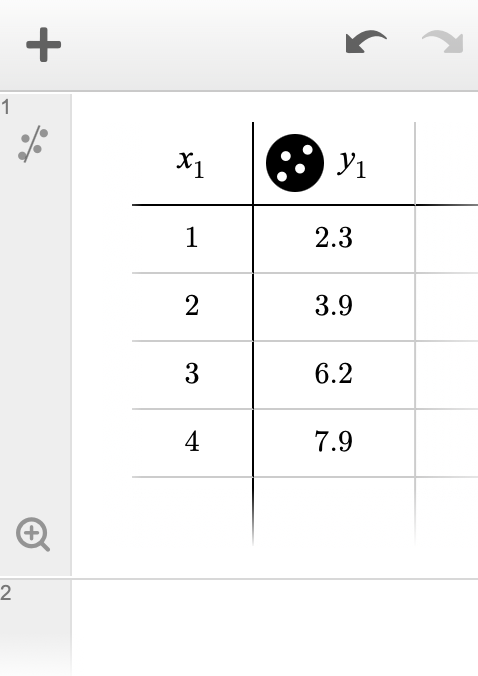
\includegraphics[width=3cm]{desmos1}};


    \node[anchor=north west] at (3.5,0) 
      {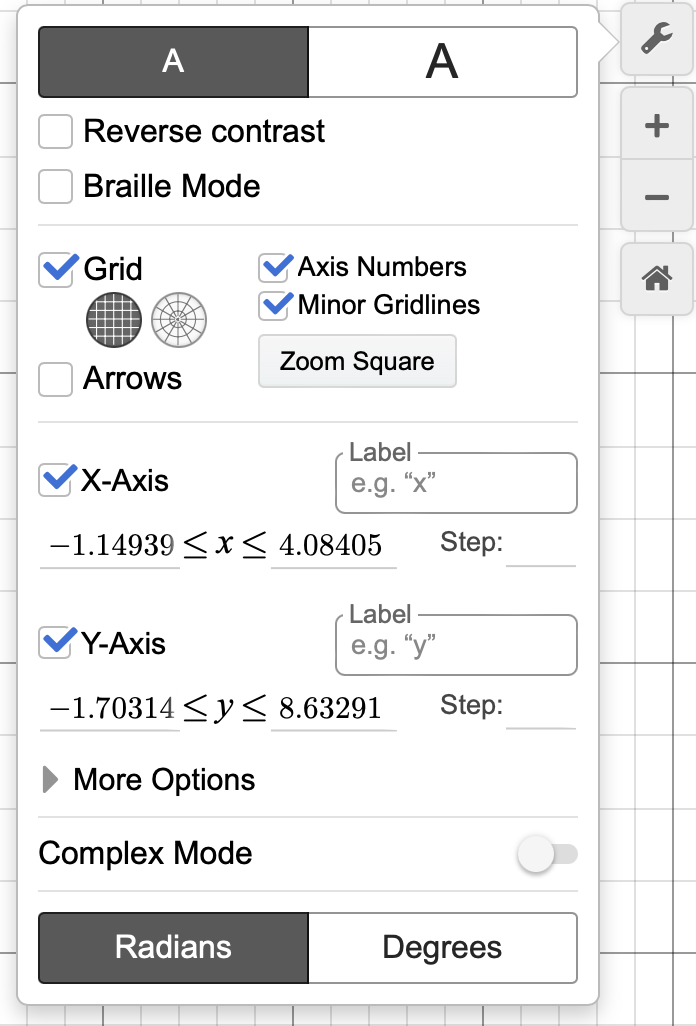
\includegraphics[width=3.5cm]{desmos2}};

        \draw (2,0) 
      node[fill=red!20,rounded corners] (table)
      {\ref{table} Create a table};
    \draw[red] (0.4,-.4) coordinate (a) circle (0.3);
    \draw[<-,red,very thick] (a) +(0.3,0) -- (table.south);

    \node[fill=blue!20,rounded corners] at (2.5,-1.5) (linear) {\ref{linear} Linear Regression};
    \draw[blue] (0.3,-1) coordinate (a) circle (0.3);
    \draw[<-,blue,very thick] (a) +(0.3,0) -- (linear.north);

    \node[fill=green!20,rounded corners] at (2,-2.5) (zoom) {\ref{zoom} Zoom Fit};
    \draw[green, ultra thick] (0.3,-3.5) coordinate (a) circle (0.3);
    \draw[<-,green,very thick] (a) +(0.3,0) -- (zoom.west);

    \node[fill=orange!20,rounded corners] at (4.5,-0.5) (wrench) {\ref{wrench} Axis Labels};
    \draw[orange, ultra thick] (6.9,-.3) coordinate (a) circle (0.3);
    \draw[<-,orange,very thick] (a) +(-0.3,0) -- (wrench.east);

    \draw[->,orange,very thick] (wrench.south) -- (5.2,-2.3);

    \draw[orange, ultra thick, rounded corners] (3.8,-2.3) rectangle ++(2.8,-0.5);
    \draw[orange, ultra thick, rounded corners] (3.8,-3.1) rectangle ++(2.8,-0.5);
  \end{tikzpicture}

\end{multicols}


  \question
    Write down the equations for each of the best fit lines below.  

    You should also copy the link to your graph, paste it on Schoology, and include the link here.

    \vspace{3em}

    Best Fit Line:

    \vspace{3em}

    Link to graph: \texttt{https://www.desmos.com/calculator/}\fillin[][10em]

    \vspace{1em}

  \question
    What is the physical meaning of the slope of your graph?
    \vs

  \question
    The expected values of the densities of each of these substances are as follows: 1.42~g/mL for honey, 0.79~g/mL for alcohol, and 0.92~g/mL for oil.  Calculate the percent error of your measured density (that is, slope).  Make sure to show your work.
    %
    \begin{align*}
      \text{\% error} &= 
      \frac{\left| 
        \text{measured} - \text{expected} 
      \right|}{
        \text{expected}
      } 
      \times 100
    \end{align*}
    %
    \vs

  \question
    Are your data accurate? Explain.
    \vs

  \question
    Are your data precise? Explain.
    \vs

\end{questions}

\end{document}